\section{Template-Based Certificate Synthesis}
\label{sec:certificate-synthesis}

The iteration-level obligations of \Cref{thm:program-rule} admit a direct
constraint-based instantiation. We implement a shared counterexample-guided
inductive synthesis (CEGIS) kernel for the random walk, FDR, and FLDR.
It searches for two independent certificates using guarded affine templates,
optionally refined by a supplied finite partition. The contribution is a
reproducible feasibility demonstration for these obligations, rather than a
new general-purpose synthesis method.

\subsection{Templates and Verification Conditions}
\label{sec:synthesis-constraints}

The input comprises integer state variables, immutable integer parameters,
a guard $b$, an initial-state description, a supplied inductive predicate
$S$, and a manually encoded complete body step. There is no program parser
or invariant synthesis. Every declared integer component is included in the
automatic feature vector $\mathbf{x}=(x_1,\ldots,x_d)$; Boolean flags may
occur in the guard but are not numerical features. Fixed numerical inputs
are substituted into the semantics. Symbolic parameters remain features.
The two templates are
\[
 V_{\mathbf a}(\sigma)=[b](\sigma)
   \Bigl(a_0+\sum_{i=1}^d a_i x_i(\sigma)\Bigr),\qquad
 U_{\mathbf u}(\sigma)=[b](\sigma)
   \Bigl(u_0+\sum_{i=1}^d u_i x_i(\sigma)\Bigr),
\]
with independent integer coefficients. The basis construction is automatic;
the supplied state representation and affine hypothesis class are not.

The paper inputs have two equiprobable complete outcomes $T_0,T_1$.
For an abstract input, an additional relation $A(\sigma,\xi)$ describes
admissible outcome pairs $T_0(\sigma,\xi),T_1(\sigma,\xi)$ using auxiliary
descriptors $\xi$, which are excluded from the feature vector. Every enabled
state must admit a pair, and every concrete outcome pair must be represented.
The latter is a separate semantic justification of the abstraction.
Suppressing $\xi$, we require on $S\land b$, for every admissible pair,
\begin{align}
 V(\sigma)&\geq1,& U(\sigma)&\geq1,
 \label{eq:syn-positive}\\
 V(T_0(\sigma))+V(T_1(\sigma))&\leq2V(\sigma),
 \label{eq:syn-supermartingale}\\
 U(T_0(\sigma))\leq U(\sigma)-1
 &\quad\lor\quad U(T_1(\sigma))\leq U(\sigma)-1,
 \label{eq:syn-progress}\\
 U(\sigma)&\leq V(\sigma).
 \label{eq:syn-domination}
\end{align}
Domination is sufficient for sublevel boundedness, but stronger than the
premise of \Cref{thm:program-rule}; integer coefficients and $V\geq1$
also restrict the search.

\begin{proposition}[Soundness of the synthesis constraints]
\label{prop:synthesis-soundness}
Suppose $S$ contains the initial states and is preserved by all represented
outcomes. If an abstraction is used, suppose it represents every concrete
outcome pair. Every instantiation satisfying
\eqref{eq:syn-positive}--\eqref{eq:syn-domination} supplies an AST
certificate with $\varepsilon=1/2$.
\end{proposition}
\begin{proof}
Both templates vanish on terminal states. On active states $V$ is positive
and $U$ is a positive integer. The expectation inequality applies to each
concrete body distribution, and at least one fair-bit outcome decreases
$U$ by one. On $V\leq r$, domination bounds $U$ by $\lfloor r\rfloor$.
Subdistributions supported in $S$ form a distributional invariant. These are
precisely the required premises of \Cref{thm:program-rule}.
\end{proof}

\subsection{Finite Search and Supplied Partitions}
\label{sec:synthesis-cegis}

For a fixed bound $B$, every coefficient ranges over $\{-B,\ldots,B\}$.
An SMT query chooses an enabled initial sample automatically, including
admissible descriptors when needed. The learner selects both coefficient
vectors simultaneously, satisfying all obligations on accumulated samples
and minimizing the sum of absolute coefficients. This objective favors
small expressions; it has no soundness role, and solver ties remain open.
The verifier fixes the coefficients and asks for any state in $S\land b$
(and admissible descriptor) violating an obligation. A satisfying assignment
is added to the samples. An unsatisfiable query verifies the candidate over
the \emph{entire} invariant domain, including unbounded integer parameters.
It is not a bounded-state test.

With a sample fixed, learner constraints are linear in the unknown
coefficients; with coefficients fixed, verifier constraints are linear in
the unknown state and descriptor variables. The supplied examples use only
Boolean combinations of linear arithmetic and piecewise affine updates.
The implementation checks initialization and preservation of $S$ separately.
For abstract inputs it also checks
$S\land b\Rightarrow\exists\xi\,A(\sigma,\xi)$; this coverage query can
contain quantification. Nonempty coverage prevents vacuous verification but
does not prove correspondence with a concrete program.

Every counterexample excludes at least the current candidate and no valid
candidate. Consequently, with exact terminating solvers and no resource
limits, the procedure terminates and is complete for a \emph{fixed finite}
template and these sufficient constraints. The implementation tries
$B=1,2,4,8,16$, retaining samples between bounds. Learner unsatisfiability
excludes only the current bounded template. Unknown results, timeouts, and
the 500-candidate limit are inconclusive. Neither the finite schedule nor
relative completeness of the proof rule establishes synthesis completeness
for AST programs.

\paragraph{Fixed piecewise affine templates.}
\label{sec:synthesis-piecewise}
The same kernel accepts a supplied partition $P_1,\ldots,P_q$ of active
invariant states, checks coverage and pairwise disjointness, and assigns an
independent full affine coefficient block to each region and each function:
\[
 V(\sigma)=[b](\sigma)\sum_{j=1}^{q}[P_j](\sigma)
 \left(a_{j,0}+\sum_{i=1}^{d}a_{j,i}x_i(\sigma)\right).
\]
The $U$-template is analogous. Predicates may use declared state components,
but not auxiliary transition descriptors or undeclared symbols. Region
selection is reevaluated at every successor, including cross-region
transitions. The constraints and soundness argument are unchanged.
A threshold split $e<r$ versus $e\geq r$ supplies both expressions;
$r$ may be a numeral or a linear expression in symbolic parameters.
Thresholds and partitions are not synthesized. Extra regions enlarge the
finite search space; they are not assumed to improve performance.

\subsection{Reproduced Results and Their Scope}
\label{sec:synthesis-examples}

\Cref{tab:synthesis-results} reports the delivered artifact run with
Z3~4.15.4 and ten seconds per solver call. The same engine, coefficient
schedule, and objective are used throughout. All final obligations are
rechecked separately. Recorded coefficient vectors, samples, counterexamples,
bound attempts, and measured wall times accompany the code; candidate counts
can vary with solver tie-breaking. These experiments are feasibility checks,
not a performance comparison with other tools.

\begin{table}[t]
\centering\small
\setlength{\tabcolsep}{4pt}
\begin{tabular}{@{}llllr@{}}
\toprule
Input & $V$ & $U$ & $B$ & Candidates\\
\midrule
Random walk & $x$ & $x$ & 1 & 2\\
FDR, symbolic $n$ & $n$ & $n-v+c$ & 1 & 3\\
FLDR, weights $(4,5)$ & $c-2d+2$ & $c-2d+2$ & 2 & 4\\
FLDR, abstract family & $m$ & $m-c$ & 1 & 4\\
Two-sided walk, supplied split & $|x|$ & $|x|$ & 1 & 4\\
\bottomrule
\end{tabular}
\caption{Synthesized expressions on active states, with terminal values zero.
$B$ is the successful bound; candidate counts include earlier bounds.
The abstract FLDR row is conditional on the structural contract below.}
\label{tab:synthesis-results}
\end{table}

\paragraph{Unbounded symmetric random walk.}
For \Cref{sec:walk}, $S\equiv x\geq0$ yields features $(x,1)$ and the
verified result $V=U=x$. The expectation is unchanged, while the left outcome
decreases $U$ by one. This establishes AST despite infinite expected runtime:
for $0<x<N$, the expected time $x(N-x)$ to hit $\{0,N\}$ lower-bounds
the time to hit $0$, and diverges with $N$.
A uniform negative expected drift is unnecessary.

\paragraph{FDR with a symbolic range.}
For the loop of \Cref{sec:fdr}, the supplied invariant is
$S\equiv n\geq1\land1\leq v<2n\land0\leq c<v\land c<n$, and the
complete bit-$\beta$ update is
\[
 T_\beta(n,v,c)=
 \begin{cases}
 (n,2v-n,2c+\beta-n),&2c+\beta\geq n,\\
 (n,2v,2c+\beta),&2c+\beta<n.
 \end{cases}
\]
The full basis $(n,v,c,1)$ yields $V=n$, $U=n-v+c$ on $v<n$,
uniformly for symbolic $n$. Put $\Delta=v-c$. Enabled states satisfy
$1\leq\Delta\leq n-1$ and $U=n-\Delta$. On bit zero a continuing
successor has $\Delta'=2\Delta$, giving $U'\leq U-1$; acceptance
sets $U'=0$. Since $n$ is unchanged, $V'$ is $n$ or zero, and $U\leq V$.
Thus an affine variant suffices in place of the manual logarithmic one.
FDR remains a baseline for the separation of certificate roles: on bit one,
$\Delta'=2\Delta-1\geq\Delta$ when continuing, so in fact
$\mathbb E[U']\leq U-1/2$. This additional inequality is independently
SMT-verified; $U$ itself is a ranking supermartingale here.

\paragraph{FLDR with fixed weights.}
For $(4,5)$, preprocessing gives $m=9$, $k=4$, and rejection weight $7$.
The artifact constructs the exact finite tree from binary weight columns,
placing internal nodes before leaves and leaf labels in descending order,
as in \Cref{sec:fldr}. The supplied invariant is its set of loop-head nodes;
the feature basis is $(c,d,1)$. After excluding $B=1$, the engine finds
$V=U=c-2d+2$ at $B=2$. \Cref{fig:fldr-synthesis-tree} displays the
five active nodes, acceptances, and resets. An independent rational-arithmetic
audit checks all nodes and edges (\Cref{app:artifact}). At the root the
expectation is unchanged, so this shared certificate has no uniform
negative drift.
\begin{figure}[tbp]
 \centering
 \begin{tikzpicture}[
   x=1cm,y=1cm,>=stealth,
   fldrnode/.style={draw=blue!55!black,fill=blue!5,rounded corners=2pt,
     minimum width=13mm,minimum height=8mm,inner sep=3pt,
     align=center,font=\small},
   fldraccept/.style={draw=teal!70!black,fill=teal!7,
     double,double distance=.5pt,rounded corners=2pt,
     minimum width=16mm,inner sep=3pt,align=center,font=\small},
   fldredge/.style={->,semithick,draw=black!75},
   fldrreset/.style={->,semithick,dashed,draw=orange!80!black,
     rounded corners=5pt},
   fldrbit/.style={font=\scriptsize,fill=white,inner sep=1.5pt}
 ]
 \node[fldrnode] (root) at (0,0) {$(0,0)$\\$W=2$};
 \node[fldrnode] (s10) at (0,-1.15) {$(1,0)$\\$W=3$};
 \node[fldrnode] (s11) at (3.5,-1.15) {$(1,1)$\\$W=1$};
 \node[fldrnode] (s20) at (0,-2.30) {$(2,0)$\\$W=4$};
 \node[fldrnode] (s30) at (0,-3.45) {$(3,0)$\\$W=5$};
 \node[fldraccept] (a22) at (2.5,-2.30)
   {Accept $2$\\$W=0$};
 \node[fldraccept] (a23) at (4.5,-2.30)
   {Accept $1$\\$W=0$};
 \node[fldraccept] (a41) at (1.25,-4.60)
   {Accept $2$\\$W=0$};

 % Each arrow includes every update of one loop-body execution.
 \draw[fldredge] (root) -- node[fldrbit,left] {$0$} (s10);
 \draw[fldredge] (root) -- node[fldrbit,above] {$1$} (s11);
 \draw[fldredge] (s10) -- node[fldrbit,left] {$0$} (s20);
 \draw[fldredge] (s11) -- node[fldrbit,pos=.58,left] {$0$} (a22);
 \draw[fldredge] (s11) -- node[fldrbit,pos=.58,right] {$1$} (a23);
 \draw[fldredge] (s20) -- node[fldrbit,left] {$0$} (s30);
 \draw[fldredge] (s30) -- node[fldrbit,above right] {$1$} (a41);

 % Reset events are contracted into their bit-labelled body transitions;
 % raw rejecting leaves are not loop-head states and get no certificate value.
 \draw[fldrreset] (s10.west) -- node[fldrbit,above] {$1$}
   (-1.20,-1.15) -- (-1.20,0) -- (root.west);
 \draw[fldrreset] (s20.west) -- node[fldrbit,above] {$1$}
   (-1.80,-2.30) -- (-1.80,.35) -- (root.north west);
 \draw[fldrreset] (s30.west) -- node[fldrbit,above] {$0$}
   (-2.40,-3.45) -- (-2.40,.75) -- (0,.75) -- (root.north);
 \node[font=\scriptsize,text=orange!80!black,rotate=90]
   at (-2.66,-1.15) {reset to $(0,0)$};

 \node[align=left,font=\small,anchor=north west,inner sep=0pt]
   at (2.65,-3.25)
   {$W=V=U=[b](c-2d+2)$\\[5pt]
    At the root:\\[2pt]
    $\mathbb E[W']=\tfrac12(3+1)=2$\\[2pt]
    $\Pr(W'<2)=\tfrac12$};
 \end{tikzpicture}
 \caption{A decision tree for FLDR with weights $(4,5)$ and rejection
 weight $7$. Active nodes show $(c,d)$ and the shared certificate value
 $W$; double-bordered leaves accept the indicated outcome and have value
 zero. Every edge represents one complete iteration with probability
 $1/2$; its label is the sampled bit. Dashed edges include rejection and
 reset, returning to the root with $W=2$. The root calculation illustrates
 progress despite zero expected decrease.}
 \label{fig:fldr-synthesis-tree}
\end{figure}

\paragraph{FLDR under a symbolic structural contract.}
For arbitrary trees, the input retains all integer components $(m,k,n,c,d)$
and uses a Boolean activity flag for the guard. Its support requires
$m\geq1$, $0\leq k\leq m$, $1\leq n\leq m$, $0\leq c\leq k$,
$d\geq0$, and $\mathit{active}\Rightarrow c<k$. Each bit outcome is
classified as continuation, rejection, or acceptance. Continuation advances
to $(c+1,2d+\beta)$ and requires $c+1<k$; rejection resets to $(0,0)$;
acceptance advances to the child and disables the guard. Parameters are
unchanged, and both outcomes may not reject simultaneously.

Tree height at most $k$ and at most one rejecting leaf per level justify
this contract (\Cref{sec:fldr}). The certificate solver does not derive these
facts from preprocessing. The domain overapproximates
$k=\lceil\log_2m\rceil$ and avoids logarithmic arithmetic.
The full basis $(m,k,n,c,d,1)$ yields $V=m$, $U=m-c$ on active states;
all irrelevant coefficients become zero without a prescribed feature subset.
Every successor has $V'$ equal to $m$ or zero, a nonrejecting outcome
decreases $U$ by at least one, and $1\leq U=m-c\leq m=V$.
The alternative pair $V=k$, $U=k-c$ is also independently verified,
but is not the candidate selected in the recorded affine run.

The depth variant can grow in expectation: at $(c,d)=(2,0)$ in the fixed
tree, $U=2$ but $\mathbb E[U']=5/2$. In the restricted basis $(k,c,1)$,
a shared function at $k=4$ has the form $W(c)=A+Dc$. Progress at the root
forces $D<0$, while its expected change at $(2,0)$ is then $-D/2>0$.
However, the synthesized $c-2d+2$ removes this obstruction. This separation
concerns a specified template class, not an intrinsic need for distinct
functions in FLDR.

\paragraph{What the supplied partition adds.}
For the symmetric walk on all of $\mathbb Z$, take guard $x\neq0$ and
support $\mathit{true}$. An affine variant $ax+b$ positive on both unbounded
tails must have $a=0$, and a constant cannot decrease at $x=2$. Hence no
single-affine pair satisfies the constraints, regardless of its coefficient
bound. With the supplied split $x<0$ versus $x\geq0$, the same kernel
synthesizes and universally verifies $V=U=|x|$. This is an expressiveness
check for a single template over the full invariant; two manual proofs on
sign-invariant domains would also suffice. Optional sampler partitions and
checks of cross-region transitions are documented in \Cref{app:artifact}.

The experiments establish neither unrestricted synthesis completeness nor
superiority to existing synthesis tools. Supplied invariants and semantics,
the FLDR abstraction, fixed partitions, and $U\leq V$ remain substantive
restrictions. Automatic extraction of semantics and partition selection are
outside the implemented scope.
